\chapter{Introduction}

\paragraph*{}
This progress report aims to highlight the progress of our final project, \textbf{Collective Transport using Swarm Robotics}, with the evaluating criteria being the team individual contributions, as well as our pace in comparison to the ideal schedule. The ideal schedule can be represented by the project Gantt Chart (Figure \ref{fig:gantt_chart}).

\paragraph*{}
According to Figure \ref{fig:gantt_chart}, we are exploring three major sub-tasks during this iteration of the project schedule. These three tasks are: \textbf{Communication in the Swarm} (Task 1.1), \textbf{Object detection using Computer Vision} (Task 1.2), and \textbf{Simple Simultaneous Localization and Mapping} (Task 1.3). These tasks are planned to span for the entire month of September. Two team members, one team member, and two team members are assigned to each task, respectively.

\begin{figure}[H]
    \centering
    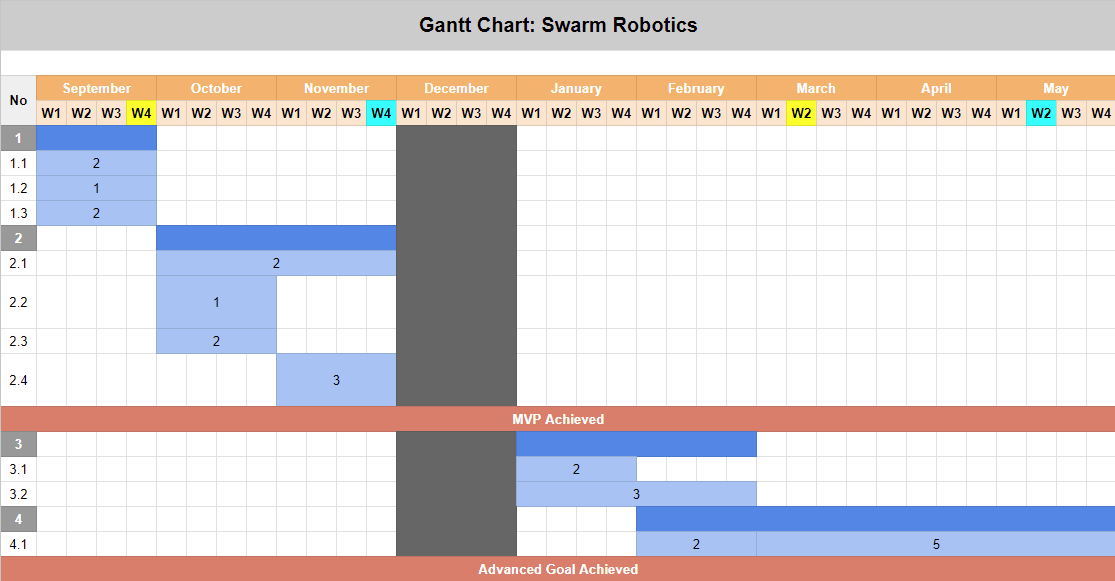
\includegraphics[width=1\linewidth]{progress_report_1/assets/images/introduction/gantt_chart.png}
    \caption{Project Gantt Chart}
    \label{fig:gantt_chart}
\end{figure}
